%iffalse
\let\negmedspace\undefined
\let\negthickspace\undefined
\documentclass[journal,12pt,onecolumn]{IEEEtran}
\usepackage[version=4]{mhchem}
\usepackage{chemformula} % for \ch if needed
\usepackage{chemfig}
\usepackage{chemmacros}
\chemsetup{modules = reactions} % Enables reaction arrows
\usepackage{graphicx}
\graphicspath{ {./images/} }

\usepackage{fancyhdr}
\usepackage{geometry}
\usepackage{lastpage}
\usepackage{cite}
\usepackage{amsmath,amssymb,amsfonts,amsthm}
\usepackage{enumitem,multicol}
\usepackage{algorithmic}
\usepackage{graphicx}
\usepackage{textcomp}
\usepackage{xcolor}
\usepackage{txfonts}
\usepackage{listings}
\usepackage{enumitem}
\usepackage{mathtools}
\usepackage{gensymb}
\usepackage{comment}
\usepackage[breaklinks=true]{hyperref}
\usepackage{tkz-euclide} 
\usepackage{listings}
\usepackage{gvv}                                        
%\def\inputGnumericTable{}                                 
\usepackage[latin1]{inputenc}                                
\usepackage{color}                                            
\usepackage{array}                                            
\usepackage{longtable}                                       
\usepackage{calc}                                             
\usepackage{multirow}                                         
\usepackage{hhline}                                           
\usepackage{ifthen}                                           
\usepackage{lscape}
\usepackage{tabularx}
\usepackage{array}
\usepackage{float}


\newtheorem{theorem}{Theorem}[section]
\newtheorem{problem}{Problem}
\newtheorem{proposition}{Proposition}[section]
\newtheorem{lemma}{Lemma}[section]
\newtheorem{corollary}[theorem]{Corollary}
\newtheorem{example}{Example}[section]
\newtheorem{definition}[problem]{Definition}
\newcommand{\BEQA}{\begin{eqnarray}}
\newcommand{\EEQA}{\end{eqnarray}}
\newcommand{\define}{\stackrel{\triangle}{=}}
\theoremstyle{remark}

\geometry{margin=1 in}

\pagestyle{fancy}

\fancyhead[C]{}
\fancyhead[L]{2023 CY}
\fancyhead[R]{\textbf{Chemistry (CY)}}
\fancyfoot[L]{CY}
\fancyfoot[C]{}
\fancyfoot[R]{\thepage/\pageref{LastPage}}

\setlength{\headheight}{14pt}
\setlength{\headsep}{5pt}
\setlength{\footskip}{20pt}


% Line thickness
\renewcommand{\headrulewidth}{0.4pt}
\renewcommand{\footrulewidth}{0.4pt}

    \usepackage{graphicx}
    \usepackage{fancyhdr}
    \pagestyle{fancy}





\begin{document}


\title{
ASSIGNMENT 5: GATE 2023 \\
CY: CHEMISTRY}
\author{AI25BTECH11021 - Abhiram Reddy N}
\maketitle


\begin{enumerate}


%----------------- Q1 ------------------
\item ``I cannot support this proposal. My ---- will not permit it.'' \hfill{\brak{\textbf{GATE CY 2023}}}
\begin{multicols}{2}
\begin{enumerate}
\item conscious
\item consensus
\item conscience
\item consent
\end{enumerate}
\end{multicols}

%----------------- Q2 ------------------
\item Courts : -----  :: Parliament : Legislature \\
(By word meaning) \hfill{\brak{\textbf{GATE CY 2023}}}
\begin{multicols}{2}
\begin{enumerate}
\item Judiciary
\item Executive
\item Governmental
\item Legal
\end{enumerate}
\end{multicols}

%----------------- Q3 ------------------
\item What is the smallest number with distinct digits whose digits add up to 45? \hfill{\brak{\textbf{GATE CY 2023}}}
\begin{multicols}{2}
\begin{enumerate}
\item 12355789
\item 123457869
\item 123456789
\item 99999
\end{enumerate}
\end{multicols}

%----------------- Q4 ------------------
\item In a class of 100 students, \hfill{\brak{\textbf{GATE CY 2023}}}

\begin{minipage}{\linewidth}
(i) there are 30 students who neither like romantic movies nor comedy movies, \\
(ii) the number of students who like romantic movies is twice the number of students who like comedy movies, and \\
(iii) the number of students who like both romantic movies and comedy movies is 20.
\end{minipage}

How many students in the class like romantic movies? 

\begin{multicols}{2}
\begin{enumerate}
\item 40
\item 20
\item 60
\item 30
\end{enumerate}
\end{multicols}


%----------------- Q5 ------------------
\item How many rectangles are present in the given figure? \hfill{\brak{\textbf{GATE CY 2023}}}
\begin{figure}
    \centering
    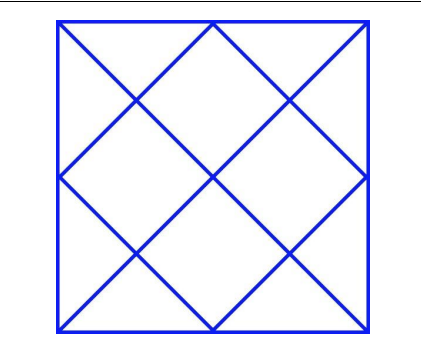
\includegraphics[width=0.3\linewidth]{figs/image1.png}
    \caption{Rectangles formed in the figure}
    \label{fig:q5_rectangles}
\end{figure}

\begin{multicols}{2}
\begin{enumerate}
\item 8
\item 9
\item 10
\item 12
\end{enumerate}
\end{multicols}



%----------------- Q6 ------------------
\item Forestland is a planet inhabited by different kinds of creatures. Among other creatures, it is populated by animals all of whom are ferocious. There are also creatures that have claws, and some that do not. All creatures that have claws are ferocious.

Based only on the information provided above, which one of the following options can be logically inferred with \textit{certainty}? \hfill{\brak{\textbf{GATE CY 2023}}}

\begin{multicols}{2}
\begin{enumerate}
\item All creatures with claws are animals.
\item Some creatures with claws are non-ferocious.
\item Some non-ferocious creatures have claws.
\item Some ferocious creatures are creatures with claws.
\end{enumerate}
\end{multicols}




%----------------- Q7 ------------------
\item Which one of the following options represents the given graph? \hfill{\brak{\textbf{GATE CY 2023}}}

\begin{figure}[H]
\centering
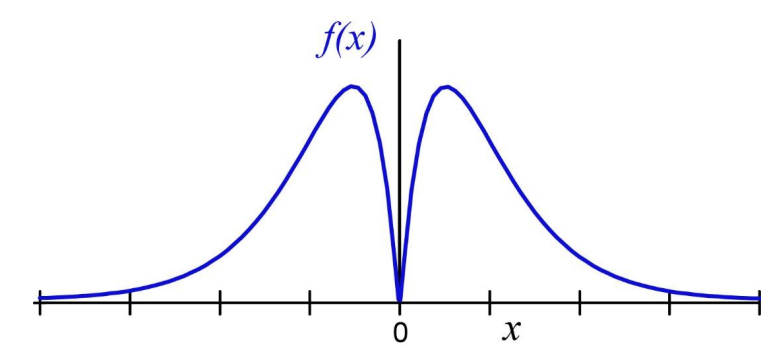
\includegraphics[width=0.5\textwidth]{figs/image2.png} 
\caption{Graph of $f(x)$ as given in the question}
\label{fig:q7graph}
\end{figure}

\begin{multicols}{2}
\begin{enumerate}
\item $f(x) = x^2 - |x|$
\item $f(x) = -x^2 + |x|$
\item $f(x) = |x^2 - x|$
\item $f(x) = x^2 - x^x$
\end{enumerate}
\end{multicols}

%----------------- Q8 ------------------
\item Which one of the following options can be inferred from the given passage alone?

\begin{quote}
When I was a kid, I was partial to stories that were about worlds and imaginary events. I would imagine that I could just get right out of space and be whisked to another planet.

\hfill{\textit{[Excerpt from The Truth about Stories by T. King]}}
\end{quote}

\hfill{\brak{\textbf{GATE CY 2023}}}

\begin{multicols}{2}
\begin{enumerate}
\item It is a child's description of what he or she likes.
\item It is an adult's memory of what he or she liked as a child.
\item The child in the passage read stories about imaginary travel only in parts.
\item It teaches us that stories are good for children.
\end{enumerate}
\end{multicols}


\newpage

%----------------- Q9 ------------------
\item Out of 1000 individuals in a town, 100 unidentified individuals are covid positive. Due to lack of adequate covid-testing kits, the health authorities of the town devised a strategy to identify these covid-positive individuals. The strategy is to:
\begin{itemize}
    \item[(i)] Collect saliva samples from all 1000 individuals and randomly group them into sets of 5.
    \item[(ii)] Mix the samples within each set and test the mixed sample for covid.
    \item[(iii)] If the test done in (ii) gives a negative result, then declare all the 5 individuals to be covid negative.
    \item[(iv)] If the test done in (ii) gives a positive result, then all the 5 individuals are separately tested for covid.
\end{itemize}

Given this strategy, no more than \rule{1cm}{0.15mm} testing kits will be required to identify all the 100 covid positive individuals irrespective of how they are grouped. \hfill{\brak{\textbf{GATE CY 2023}}}

\begin{multicols}{2}
\begin{enumerate}
\item 700
\item 600
\item 800
\item 1000
\end{enumerate}
\end{multicols}

%----------------- Q10 ------------------
\item A 100 cm * 32 cm rectangular sheet is folded 5 times. Each time the sheet is folded, the long edge aligns with its opposite side. Eventually, the folded sheet is a rectangle of dimensions 100 cm * 1 cm.

The total number of creases visible when the sheet is unfolded is \rule{1cm}{0.15mm}. \hfill{\brak{\textbf{GATE CY 2023}}}

\begin{multicols}{2}
\begin{enumerate}
\item 32
\item 5
\item 31
\item 63
\end{enumerate}
\end{multicols}













%----------------- Q11 ------------------
\item The major product formed in the following reaction is \hfill{\brak{\textbf{GATE CY 2023}}}

\begin{figure}[h!]
    \centering
    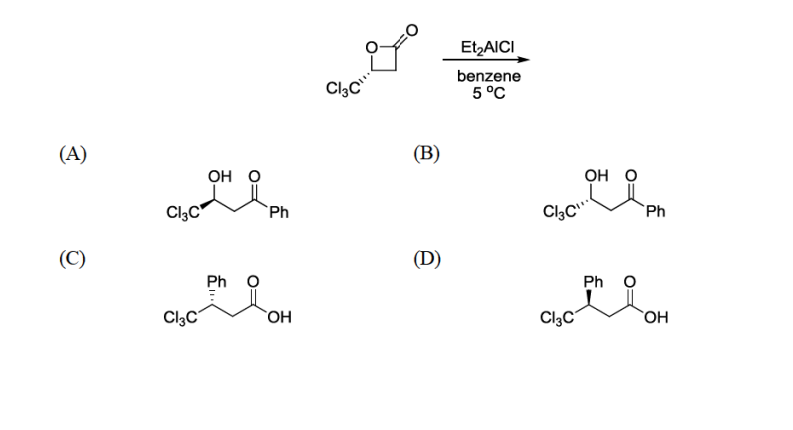
\includegraphics[width=0.9\textwidth]{figs/image5.png}
    \caption{Reaction for Q11}
    \label{fig:q11reaction}
\end{figure}

\newpage

%----------------- Q12 ------------------
\item In the following reaction, the stereochemistry of the major product is predicted by the \hfill{\brak{\textbf{GATE CY 2023}}}

\begin{figure}[h!]
    \centering
    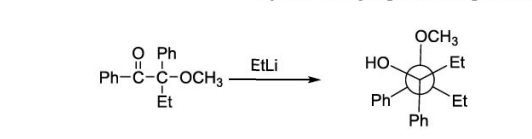
\includegraphics[width=0.9\textwidth]{figs/image6.png}
    \caption{Reaction for Q12}
    \label{fig:q12reaction}
\end{figure}

\begin{multicols}{2}
\begin{enumerate}
    \item Cram's model
    \item Cram's chelation model
    \item Felkin model
    \item Felkin-Ahn model
\end{enumerate}
\end{multicols}

%----------------- Q13 ------------------
\item The product(s) formed in the following reaction is (are) \hfill{\brak{\textbf{GATE CY 2023}}}

\begin{figure}[h!]
    \centering
    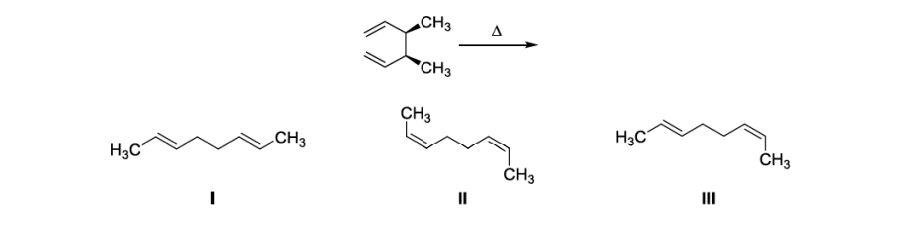
\includegraphics[width=0.8\textwidth]{figs/image7.png}
    \caption{Reaction for Q13}
    \label{fig:q13reaction}
\end{figure}

\begin{multicols}{2}
\begin{enumerate}
    \item I only
    \item II only
    \item III only
    \item mixture of I and II
\end{enumerate}
\end{multicols}
\newpage
%----------------- Q14 ------------------
\item Among the following compounds, the number of compounds that DO NOT exhibit optical activity at room temperature is \hfill{\brak{\textbf{GATE CY 2023}}}

\begin{figure}[h!]
    \centering
    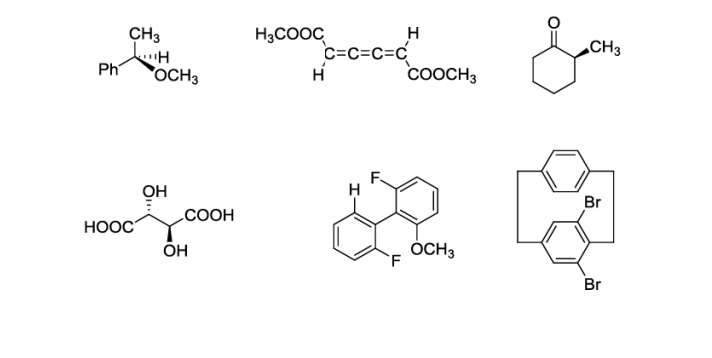
\includegraphics[width=0.8\textwidth]{figs/image8.png}
    \caption{Compounds for Q14}
    \label{fig:q14compounds}
\end{figure}





%----------------- Q15 ------------------
\item The number of following diene(s) that undergo Diels-Alder reaction with methyl acrylate is \hfill{\brak{\textbf{GATE CY 2023}}}

\begin{figure}[h!]
    \centering
    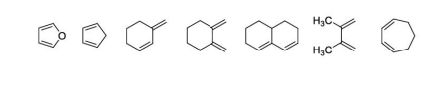
\includegraphics[width=0.8\textwidth]{figs/image9.png}
    \caption{Dienes for Q15}
    \label{fig:q15dienes}
\end{figure}

%----------------- Q16 ------------------
\item The number of \(^1H\) NMR signals observed for the following compound is \hfill{\brak{\textbf{GATE CY 2023}}}

\begin{figure}[h!]
    \centering
    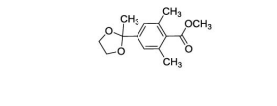
\includegraphics[width=0.6\textwidth]{figs/image10.png}
    \caption{Compound for Q16}
    \label{fig:q16compound}
\end{figure}

\newpage
%----------------- Q17 ------------------
\item The number of CO stretching bands in IR spectrum of trigonal bipyramidal \textit{cis}-M(CO)$_3$L$_2$ is \hfill{\brak{\textbf{GATE CY 2023}}}

(M = metal and L = monodentate ligand)

%----------------- Q18 ------------------
\item On heating a sample of 25 mg hydrated compound (molecular weight = 250 g/mol) in thermogravimetric analysis, 16 mg of dehydrated compound remains. The number of water molecules lost per molecule of hydrated compound is \hfill{\brak{\textbf{GATE CY 2023}}}

(Molecular weight of water = 18 g/mol)

%----------------- Q19 ------------------
\item The total number of $\alpha$ and $\beta$ particles emitted in the following radioactive decay is \hfill{\brak{\textbf{GATE CY 2023}}}

\begin{figure}[h!]
    \centering
    
\includegraphics[width=0.6\textwidth]{figs/image11.png}
    \caption{Radioactive decay for Q19}
    \label{fig:q19decay}
\end{figure}






%----------------- Q20 ------------------
\item An ideal gas occupies an unknown volume \(V\) liters (L) at a pressure of 12 atm. The gas is expanded isothermally against a constant external pressure of 2 atm so that its final volume becomes 31 L. The work involved for this expansion process is cal. (Round off to two decimal places) \hfill{\brak{\textbf{GATE CY 2023}}}

(Gas constant \(R = 0.082 \text{ L atm mol}^{-1} \text{K}^{-1} 2 \text{ cal mol}^{-1} \text{K}^{-1}\))

%----------------- Q21 ------------------
\item The entropy change for the melting of \(x\) moles of ice (heat of fusion is 80 cal g\(^{-1}\)) at 273 K and 1 atm pressure is 28.80 cal K\(^{-1}\). The value of \(x\) is . (Round off to two decimal places)

(Molecular weight of water = 18 g/mol) \hfill{\brak{\textbf{GATE CY 2023}}}

%----------------- Q22 ------------------
\item Consider a two-state system at thermal equilibrium having energies 0 and 2\(kT\) for which the degeneracies are 1 and 2, respectively. The value of the partition function at the same absolute temperature T is . (Round off to two decimal places)

(\(k\) is the Boltzmann constant) \hfill{\brak{\textbf{GATE CY 2023}}}

%----------------- Q23 ------------------
\item Consider a system of three identical and cistriglyceride non-interacting particles and three available nondegenerate single particle energy levels having energies 0, 0, and 2\(\epsilon\). The system is in contact with a heat bath of temperature \(T\). A total energy of 2\(\epsilon\) is shared by these three particles. The number of ways five particles can be distributed is . \hfill{\brak{\textbf{GATE CY 2023}}}

%----------------- Q24 ------------------
\item In a 400 MHz \(^1H\) NMR spectrometer, a proton resonates at 1560 Hz higher than that of tetramethylsilane. The chemical shift value of this proton is  ppm. (Round off to one decimal place)

(Chemical shift of tetramethylsilane is fixed at zero ppm) \hfill{\brak{\textbf{GATE CY 2023}}}

%----------------- Q25 ------------------
\item Gas phase bond length and dipole moment of a compound (MX) is 3 A and 10.8 D, respectively. The ionic character in gas phase MX is  %. (Round off to one decimal place)

(1 D = 3.336 \(\times 10^{-30}\) C m) \hfill{\brak{\textbf{GATE CY 2023}}}





%----------------- Q26 ------------------
\item The experimentally observed magnetic moment values, which match well with the spin-only values for the pair of argon ions is \hfill{\brak{\textbf{GATE CY 2023}}}
\begin{multicols}{2}
\begin{enumerate}
\item  Cr(III) and Cr(II)
\item  Cr(III) and Cr(III)
\item  Cr(III) and Dy(III)
\item  La(III) and Tb(III)
\end{enumerate}
\end{multicols}




%----------------- Q27 ------------------
\item Point group of naphthalene (\ce{C10H8}) is \hfill{\brak{\textbf{GATE CY 2023}}}

\begin{multicols}{2}
\begin{enumerate}
\item \ce{D_{2h}}
\item \ce{D_{2d}}
\item \ce{D_{2}}
\item \ce{D_{10h}}
\end{enumerate}
\end{multicols}

%----------------- Q28 ------------------
\item The \textbf{INCORRECT} statement is \hfill{\brak{\textbf{GATE CY 2023}}}

\begin{multicols}{1}
\begin{enumerate}
\item Zero-point energy of a quantum mechanical harmonic oscillator of frequency \(\nu\) is \(h\nu/2\)
\item Energy level of a quantum mechanical rigid rotor is inversely proportional to its moment of inertia
\item The time-independent Schrödinger equation for \(L^2\) operator has no exact solution
\item Total angular momentum of an atomic system is equal to the sum of orbital angular momentum and spin angular momentum
\end{enumerate}
\end{multicols}

%----------------- Q29 ------------------
\item For an ideal gas, the molecular partition function in the canonical ensemble, that is proportional to the system volume (V), is the \hfill{\brak{\textbf{GATE CY 2023}}}

\begin{multicols}{2}
\begin{enumerate}
\item vibrational partition function
\item rotational partition function
\item electronic partition function
\item translational partition function
\end{enumerate}
\end{multicols}

%----------------- Q30 ------------------
\item Assertion (A): The total angular momentum for light atoms (low atomic number) is obtained through Russell-Saunders coupling, wherein coupling is more of heavy nuclei through j-j coupling.\\
Reason (R): The spin-orbit interaction is weak in light atoms (low atomic number) because they have weak electric fields. \hfill{\brak{\textbf{GATE CY 2023}}}

\begin{multicols}{1}
\begin{enumerate}
\item A and R are true, and R is the correct reason for A
\item A and R are true, but R is NOT the correct reason for A
\item A is true but R is false
\item A is false but R is true
\end{enumerate}
\end{multicols}








%----------------- Q31 ------------------
\item The correct molecular representation of W(Cp)$_2$(CO)$_2$ is \hfill{\brak{\textbf{GATE CY 2023}}}

\begin{enumerate}
\item [(A)] [W($\eta^1$-Cp)($\eta^3$-Cp)(CO)$_2$]
\item [(B)] [W($\eta^1$-Cp)($\eta^5$-Cp)(CO)$_2$]
\item [(C)] [W($\eta^3$-Cp)($\eta^5$-Cp)(CO)$_2$]
\item [(D)] [W($\eta^5$-Cp)$_2$(CO)$_2$]
\end{enumerate}




%----------------- Q32 ------------------
\item Match the metalloproteins with their respective functions. \hfill{\brak{\textbf{GATE CY 2023}}}

\begin{center}
\begin{tabular}{|c|c|c|c|}
\hline
P & Ferritin & I & Electron transfer \\
Q & Rubredoxin & II & Acid-base catalysis \\
R & Cobalamin & III & Metal storage \\
S & Carbonic anhydrase & IV & Methyl transfer \\
\hline
\end{tabular}
\end{center}

\begin{multicols}{2}
\begin{enumerate}
\item [(A)] P - III; Q - II; R - I; S - IV
\item [(B)] P - III; Q - I; R - IV; S - II
\item [(C)] P - IV; Q - I; R - III; S - II
\item [(D)] P - IV; Q - II; R - I; S - III
\end{enumerate}
\end{multicols}

\newpage


%----------------- Q33 ------------------
\item Suppose the wave function of a one dimensional system is 
\[
\psi = \sin(kx) \exp(3ikx).
\]
In an experiment measuring the momentum of the system, one of the expected outcomes is \hfill{\brak{\textbf{GATE CY 2023}}}
\begin{multicols}{4}
\begin{enumerate}
\item 0
\item $\hbar k$
\item $2 \hbar k$
\item $3 \hbar k$
\end{enumerate}
\end{multicols}



%----------------- Q34 ------------------
\item For the Lindemann-Hinshelwood mechanism of gas phase unimolecular reactions, the true statement(s) is(are) \hfill{\brak{\textbf{GATE CY 2023}}}

\begin{multicols}{1}
\begin{enumerate}
\item Only molecules with three or more atoms can follow the Lindemann-Hinshelwood mechanism
\item Lindemann-Hinshelwood mechanism involves bimolecular elementary steps
\item The overall reaction is of second order at low pressure
\item The overall reaction is of second order at high pressure
\end{enumerate}
\end{multicols}

%----------------- Q35 ------------------
\item The calculated magnetic moment of [Ce(NO\textsubscript{3})\textsubscript{3}]\textsuperscript{2-} is -----BM. (rounded off to two decimal places) \hfill{\brak{\textbf{GATE CY 2023}}}

(Given: atomic number of Ce is 58)







%----------------- Q36 ------------------
\item The major product formed in the following reaction is \hfill{\brak{\textbf{GATE CY 2023}}}

\begin{figure}[H]
    \centering
    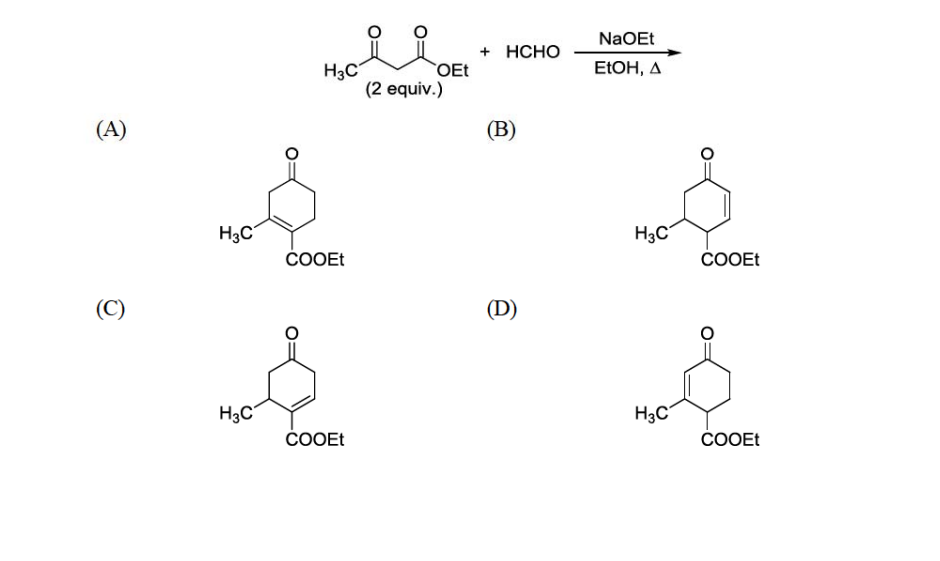
\includegraphics[width=0.8\linewidth]{figs/image14.png}
    \caption{Reaction for Q36}
    \label{fig:q36}
\end{figure}


%----------------- Q37 ------------------
\item The major product formed in the following reaction is \hfill{\brak{\textbf{GATE CY 2023}}}

\begin{figure}[H]
    \centering
    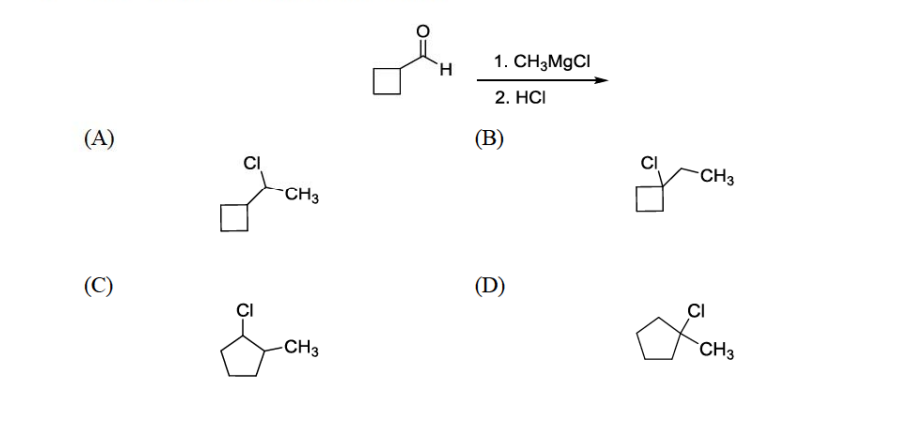
\includegraphics[width=0.8\linewidth]{figs/image15.png}
    \caption{Reaction for Q37}
    \label{fig:q37}
\end{figure}



%----------------- Q38 ------------------
\item In the following reaction sequence, the products \textit{P} and \textit{Q} are \hfill{\brak{\textbf{GATE CY 2023}}}

\begin{figure}[H]
    \centering
    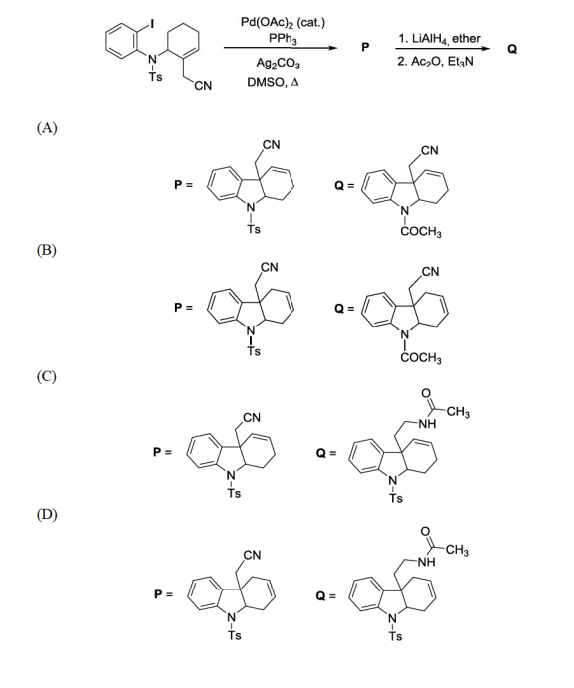
\includegraphics[width=0.6\linewidth]{figs/image16.png}
    \caption{Reaction sequence for Q38}
    \label{fig:q38}
\end{figure}



%----------------- Q39 ------------------
\item The major product formed in the following reaction is \hfill{\brak{\textbf{GATE CY 2023}}}

\begin{figure}[H]
    \centering
    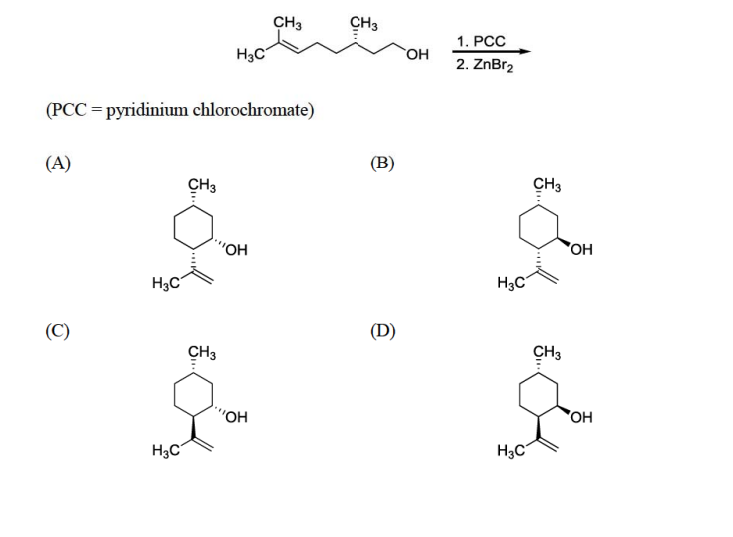
\includegraphics[width=0.8\linewidth]{figs/image17.png}
    \caption{Reaction for Q39}
    \label{fig:q39}
\end{figure}





%----------------- Q40 ------------------
\item In the $^{1}$H NMR spectrum, multiplicity of the signal (bold and underlined H atom) in the following species is
\begin{multicols}{2}
\begin{enumerate}
\item[(I)] \textbf{\underline{H}}Ni(OPEt$_3$)$_4$]$^{+}$
\item[(II)] Ph$_2$Si(Me)\textbf{\underline{H}}
\item[(III)] PH$_3$
\item[(IV)] (Cp*)$_2$ZrH\textbf{\underline{2}} (Cp* = pentamethylcyclopentadienyl)
\end{enumerate}
\end{multicols}

\begin{multicols}{2}
\begin{enumerate}
\item I- pentet, II- quartet, III- doublet and IV- singlet
\item I- pentet, II- singlet, III- singlet and IV- doublet
\item I- triplet, II- triplet, III- doublet and IV- doublet
\item I- singlet, II- quartet, III- singlet and IV- singlet
\end{enumerate}
\end{multicols}

%----------------- Q41 ------------------
\item The major product obtained by the treatment of (η$^{5}$-C$_5$H$_5$)$_2$Ni with Na/Hg in ethanol is
\begin{multicols}{2}
\begin{enumerate}
\item (η$^{5}$-C$_5$H$_5$)(η$^{3}$-C$_5$H$_5$)Ni
\item (η$^{3}$-C$_5$H$_5$)$_2$Ni
\item (η$^{5}$-C$_5$H$_5$)(η$^{3}$-C$_5$H$_7$)Ni
\item (η$^{3}$-C$_5$H$_7$)$_2$Ni
\end{enumerate}
\end{multicols}




%----------------- Q42 ------------------
\item The number of shared corners of the constituent SiO$_4$ units in orthosilicate, pyrosilicate, cyclic silicate and sheet silicate, respectively, are
\begin{multicols}{2}
\begin{enumerate}
\item 0, 1, 2 and 3
\item 2, 3, 0 and 1
\item 0, 3, 1 and 2
\item 1, 2, 3 and 0
\end{enumerate}
\end{multicols}


\newpage
%----------------- Q43 ------------------
\item Concentration of Q in a consecutive reaction 
\[
P \xrightarrow{k_1} Q \xrightarrow{k_2} R
\]
is given by
\[
[Q] = \frac{k_1[P]_0}{k_2 - k_1} \left[ e^{-k_1 t} - e^{-k_2 t} \right],
\]
where $[P]_0$ is the initial concentration of P.

If the value of $k_2 = 25$ s$^{-1}$, the value of $k_1$ that leads to the longest waiting time for Q to reach its maximum is
\begin{multicols}{2}
\begin{enumerate}
\item $k_1 = 20$ s$^{-1}$
\item $k_1 = 25$ s$^{-1}$
\item $k_1 = 30$ s$^{-1}$
\item $k_1 = 35$ s$^{-1}$
\end{enumerate}
\end{multicols}



%----------------- Q44 ------------------
\item The wavefunction for Be$^{2+}$ in a certain state is given by 
\[
\psi = N e^{-\frac{r}{a_0}},
\]
where $N$ is the normalization constant, $r$ is the distance of electron from the nucleus and $a_0$ is the Bohr radius. The most probable distance of the electron from the nucleus in this state is
\begin{multicols}{2}
\begin{enumerate}
\item $4a_0$
\item $\frac{a_0}{4}$
\item $8a_0$
\item $\frac{a_0}{8}$
\end{enumerate}
\end{multicols}

%----------------- Q45 ------------------
\item Match the following

\begin{tabular}{ll}
\textbf{Column I} & \textbf{Column II} \\
(P) Associated Legendre polynomials & (I) Harmonic oscillator \\
(Q) Hermite polynomials & (II) Particle in a box model \\
(R) Associated Laguerre polynomials & (III) Angular part of H atom \\
(S) Trigonometric functions & (IV) Radial part of H atom \\
\end{tabular}

\begin{multicols}{2}
\begin{enumerate}
\item P $\rightarrow$ III, Q $\rightarrow$ I, R $\rightarrow$ IV, S $\rightarrow$ II
\item P $\rightarrow$ III, Q $\rightarrow$ IV, R $\rightarrow$ II, S $\rightarrow$ I
\item P $\rightarrow$ IV, Q $\rightarrow$ I, R $\rightarrow$ III, S $\rightarrow$ II
\item P $\rightarrow$ II, Q $\rightarrow$ III, R $\rightarrow$ IV, S $\rightarrow$ I
\end{enumerate}
\end{multicols}



%----------------- Q46 ------------------
\item In the scheme below,
\begin{figure}[H]
    \centering
    \[
    \mathrm{P_2} \xleftrightarrow[k_1]{I_a} 2Q \xrightarrow{k_2} R
    \]
    \caption{Reaction scheme showing conversion of $\mathrm{P_2}$ to $2Q$ and then to $R$.}
    \label{fig:Q46_scheme}
\end{figure}

$I_a$ represents the intensity of the light absorbed. Assuming that the quantum yield of the first step is one, the steady state concentration of Q is given by

\begin{multicols}{2}
\begin{enumerate}
\item $\sqrt{\frac{I_a}{k_1 + k_2}}$
\item $\sqrt{\frac{I_a[P_2]}{k_1 + k_2}}$
\item $\frac{I_a}{k_1 + k_2}$
\item $\frac{I_a[P_2]}{k_1 + k_2}$
\end{enumerate}
\end{multicols}



%----------------- Q47 ------------------
\item Consider the following two parallel irreversible first order reactions at temperature T, \hfill{\brak{\textbf{GATE CY 2023}}}

\begin{figure}[H]
    \centering
    
\includegraphics[width=0.7\linewidth]{figs/image22.png}
    \caption{Reaction scheme for Q47}
    \label{fig:q47}
\end{figure}

\noindent where \(k_1\) and \(k_2\) are the rate constants and their values are \(5 \times 10^{-2}~\text{min}^{-1}\) and \(15 \times 10^{-2}~\text{min}^{-1}\), respectively, at temperature T. If the initial concentration of the reactant \(P\) is \(4~\text{mol L}^{-1}\), then the concentration of product \(R\) after 10 min of reaction is \rule{2cm}{0.15mm} mol L\(^{-1}\). (Round off to two decimal places)

\textbf{(Assume only P is present at the beginning of the reaction.)}

%----------------- Q48 ------------------
\item Consider the following equilibrium \hfill{\brak{\textbf{GATE CY 2023}}}

\[
\text{SO}_2 (g) + \frac{1}{2} \text{O}_2 (g) \rightleftharpoons \text{SO}_3 (g)
\]

At 298 K, the standard molar Gibbs energies of formation, \(\Delta G_f^\circ\), of SO\(_2\) (g) and SO\(_3\) (g) are -300 and -371 kJ mol\(^{-1}\), respectively. The value of the equilibrium constant, \(K_p\), at this temperature is \rule{2cm}{0.15mm} \(\times 10^{10}\). (Round off to the nearest integer)

\textbf{(Gas constant R = 8.31 J mol\(^{-1}\) K\(^{-1}\))}




%----------------- Q49 ------------------
\item Consider the electrochemical cell
\[
\text{M(s)}|\text{M}^{2+}(s)|\text{M}|\text{M(s)}
\]
where `M' is a metal. At 298 K, the standard reduction potentials are 
\[
E^\circ_{\text{M}^{2+}(aq)/M(s)} = -0.12~V, \quad
E^\circ_{\text{M}^{2+}_{(s)}/M(s)} = -0.36~V
\]
and the temperature coefficient is
\[
\left(\frac{\partial E^\circ_{\text{cell}}}{\partial T}\right)_P = 1.5 \times 10^{-4} \, V\,K^{-1}.
\]
At this temperature the standard enthalpy change for the overall cell reaction, \(\Delta_r H^\circ\), is \rule{2cm}{0.15mm} kJ mol\(^{-1}\). (Round off to two decimal places)

(Faraday constant F = 96500 C mol\(^{-1}\))

%----------------- Q50 ------------------
\item The normal boiling point of a compound (X) is 350 K (heat of vaporization, \(\Delta_{vap}H_v = 30\) kJ mol\(^{-1}\)). The pressure required to boil 'X' at 300 K is \rule{2cm}{0.15mm} Torr. (Round off to two decimal places)

(Ignore the temperature variation of \(\Delta_{vap}H_v\); Gas constant R = 8.31 J mol\(^{-1}\) K\(^{-1}\) and 1 atm = 760 Torr)

\newpage


%----------------- Q51 ------------------
\item For a bimolecular gas phase reaction \(P + Q \rightarrow R\), the pre-exponential factor is \(1 \times 10^{13}\) dm\(^3\) mol\(^{-1}\) s\(^{-1}\). The standard entropy of activation at 25 \(^{\circ}\)C is \rule{2cm}{0.15mm} J K\(^{-1}\) mol\(^{-1}\). (Round off to two decimal points)

(The standard concentration \(c^\circ = 1\) mol dm\(^{-3}\); Planck constant \(h = 6.62 \times 10^{-34}\) J s; Boltzmann constant \(k_B = 1.38 \times 10^{-23}\) J K\(^{-1}\); Gas constant \(R = 8.31\) J mol\(^{-1}\) K\(^{-1}\))




%----------------- Q52 ------------------
\item The correct statement(s) regarding myoglobin (Mb) and haemoglobin (Hb) is(are)
\begin{multicols}{2}
\begin{enumerate}
\item At low partial pressure of O$_2$ (e.g., 5 kPa), the O$_2$ affinity of Hb lowers upon lowering the pH
\item Binding of the first O$_2$ molecule to Hb results in lower affinity for the binding of second O$_2$ molecule
\item Metal center in deoxy-Mb is low-spin whereas it is high-spin in the case of oxy-Mb
\item One end of O$_2$ binds to the metal center in oxy-Mb and the other end of the bound O$_2$ is H-bonded with imidazole-NH of a distal histidine
\end{enumerate}
\end{multicols}

%----------------- Q53 ------------------
\item The correct statement(s) regarding Co$_2$(CO)$_8$ is(are)
\begin{multicols}{2}
\begin{enumerate}
\item It reacts with Na to give Na[Co(CO)$_4$]
\item It contains three bridging carbonyls
\item It can be prepared by reductive carbonylation of Co(OAc)$_2\cdot$4H$_2$O
\item Two isomers exist in hexane solution
\end{enumerate}
\end{multicols}



%----------------- Q54 ------------------
\item The compound(s) having [Xe]4f$^1$ configuration is(are) \\
(Given the atomic numbers Ce:58, Lu:71, Pr:59 and Nd:60)
\begin{multicols}{2}
\begin{enumerate}
\item Na$_3$[Ce(NO$_3$)$_6$]
\item Na$_3$[LuCl$_6$]
\item PrO$_2$
\item Nd(NR$_2$)$_3$ (R = SiMe$_3$)
\end{enumerate}
\end{multicols}

%----------------- Q55 ------------------
\item The correct statement(s) for XeF$_2$ is(are)
\begin{multicols}{2}
\begin{enumerate}
\item Its bonding is best explained by classical 2-centered-2-electron bonds
\item Its bonding is best explained by a non-classical 3-centered-4-electron bond
\item It contains nine lone pairs of electrons
\item Its point group is $D_{\mathrm{oxh}}$
\end{enumerate}
\end{multicols}




%----------------- Q56 ------------------
\item For the non-dissociative adsorption of a gas on solid, \\
(i) the Freundlich isotherm is given by $b = kp^n$ where $\theta$ is surface coverage, $p$ is pressure, $k$ and $n$ are empirical constants; and \\
(ii) the BET isotherm is given by 
\[
\frac{p}{p_0 - p} = \frac{1}{cp} + \frac{c-1}{c} \left(\frac{p}{p_0}\right)
\]
where $p^*$ and $c$ are empirical constants, and $p < p^*$. \\
The correct statement(s) is(are)
\begin{multicols}{2}
\begin{enumerate}
\item At low surface coverage, the Langmuir isotherm reduces to the Freundlich isotherm with $n=1$
\item At high surface coverage, the Langmuir isotherm reduces to the Freundlich isotherm with $n = \infty$
\item At very low pressure ($p \ll p^*$), the BET isotherm reduces to the Langmuir isotherm
\item At very high pressure ($p \sim p^*$), the BET isotherm reduces to the Freundlich isotherm
\end{enumerate}
\end{multicols}

%----------------- Q57 ------------------
\item Two different enzyme catalysis reactions I and II have identical Y-intercepts for the Lineweaver-Burke (equation given below) plots. The slope for reaction I is twice than that of reaction II. \\
If the initial concentrations of enzymes in I and II are same, the correct statement(s) is(are) \\
\[
\frac{1}{v} = \frac{1}{v_{\max}} + \frac{K_m}{v_{\max}} \frac{1}{[S]}
\]
where $v$ and $v_{\max}$ are rate and maximum rate; $K_m$ is Michaelis-Menten constant, and $[S]$ is substrate concentration.
\begin{multicols}{2}
\begin{enumerate}
\item Reactions I and II have same turn over number
\item Michaelis-Menten constants for reactions I and II are identical
\item Michaelis-Menten constant for reaction I is twice than that of reaction II
\item The rates of the elementary steps for reactions I and II are identical
\end{enumerate}
\end{multicols}




%----------------- Q58 ------------------
\item The enthalpy change for the exothermic reaction between BeI$_2$ and HgF$_2$ is----- kJ mol$^{-1}$ (rounded off to the nearest integer) \\
(Given: Bond dissociation energy (in kJ mol$^{-1}$) for Be-F = 632, Be-I = 289, Hg-F = 268 and Hg-I = 145)

%----------------- Q59 ------------------
\item Number of carbon atoms connected to the metal center in [W(C$_6$)(CO)$_5$] is ----- (rounded off to the nearest integer) \\
(Given: atomic number of W is 74)

%----------------- Q60 ------------------
\item Two-component solid-liquid system of naphthalene-benzene forms a simple eutectic mixture. Assuming that naphthalene-benzene forms an ideal solution, the mole fraction of naphthalene in benzene at 300 K and 1 bar is ----- (rounded off to two decimal places) \\
(Given: Freezing point ($T_f^0$) and enthalpy of fusion ($\Delta H_f^0$) of naphthalene are 353 K and 19.28 kJ mol$^{-1}$, respectively and gas constant ($R$) = 8.31 J K$^{-1}$ mol$^{-1}$)

%----------------- Q61 ------------------
\item The intrinsic viscosity of a sample of polystyrene in toluene is 84 cm$^3$ g$^{-1}$ at 30 $^\circ$C. It follows Mark-Houwink equation with empirical constant values of $K = 1.05 \times 10^{-2}$ cm$^3$ g$^{-1}$ and $a = 0.75$. The molecular weight of the polymer is ----- $\times 10^3$ g mol$^{-1}$ (rounded off to the nearest integer)

%----------------- Q62 ------------------
\item According to Debye-Huckel limiting law, the mean molal activity coefficient for 0.87 g K$_2$SO$_4$ (molar mass = 174 g mol$^{-1}$) in 1 kg of water at 25 $^\circ$C is ----- (rounded off to two decimal places)

\newpage



%----------------- Q63 ------------------
\item A solution is prepared by dissolving 128 g of naphthalene (C$_{10}$H$_8$) in 780 g of benzene (C$_6$H$_6$). The vapor pressure of pure benzene is 12.6 kPa at 25 $^\circ$C. Assuming that naphthalene in benzene is an ideal solution, the partial vapor pressure of benzene is ------kPa (rounded off to two decimal places)

%----------------- Q64 ------------------
\item For the galvanic cell: H$_2$ (g) | HCl (aq) | Cl$_2$ (g) \\
the standard electromotive force ($E^0$) value is given by
\[
E^0 = 1.73 - (1.25 \times 10^{-3})T + (1.00 \times 10^{-6})T^2
\]
where $E^0$ is in Volts and $T$ is in Kelvin. \\
For the cell reaction, the standard enthalpy change ($\Delta_r H^0$) at 300 K is ------ kJ mol$^{-1}$ (rounded off to the nearest integer) \\
(Given: Faraday constant, $F = 96500$ C mol$^{-1}$)

%----------------- Q65 ------------------
\item A solution of three non-interacting compounds P, Q, and R is taken in a cuvette of 1 cm path length. Their concentrations are [P] = $1 \times 10^{-6}$ M, [Q] = $2 \times 10^{-6}$ M, [R] = $3 \times 10^{-6}$ M and the molar extinction coefficients at 300 nm are $\varepsilon_P = 1 \times 10^{5}$ M$^{-1}$ cm$^{-1}$, $\varepsilon_Q = 2 \times 10^{5}$ M$^{-1}$ cm$^{-1}$ and $\varepsilon_R = 3 \times 10^{5}$ M$^{-1}$ cm$^{-1}$. The \% transmittance at 300 nm is ------ (rounded off to two decimal places)

\end{enumerate}

\vspace{3 cm}


\begin{center}
    \textbf{END OF THE QUESTION PAPER}
\end{center}

\end{document}